\section{eplusmap.\textless{}ext\textgreater{}}\label{eplusmap.ext}

The eplusmap.csv (or txt or tab extension) is a file that is generated by the Output:IlluminanceMap object. These are calculated for the Daylighting:Controls daylighting option. By default, this is a comma delimited text file (csv) that can be imported into a spreadsheet program. For example, the input for the Output:IlluminanceMap object shown below:

\begin{lstlisting}
Output:IlluminanceMap,
    Daylit Map,              !- Map Name
    Daylit Zone,             !- Zone Name
    0.8,                     !- Z height {m}
    0.1,                     !- X minimum coordinate {m}
    4.9,                     !- X maximum coordinate {m}
    10,                      !- Number of X grid points
    0.1,                     !- Y minimum coordinate {m}
    9.9,                     !- Y maximum coordinate {m}
    10;                      !- Number of Y grid points
\end{lstlisting}

generates the following output in csv format when viewed with Microsoft Excel.~ \textbf{Note that if the point is outside the zone a ``*'' will be shown.}

\begin{figure}[hbtp] % fig 7
\centering
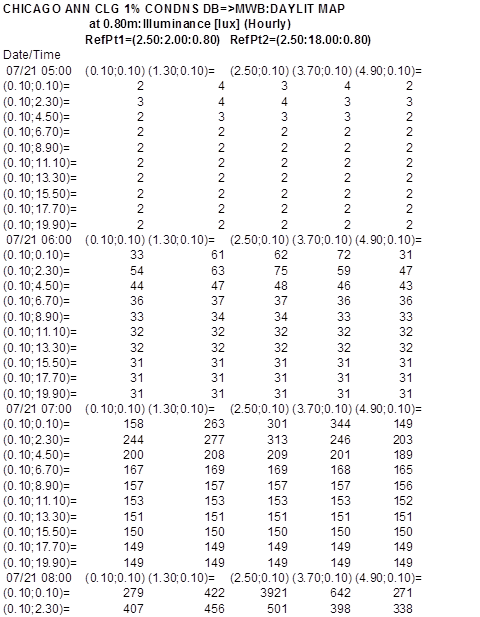
\includegraphics[width=0.9\textwidth, height=0.9\textheight, keepaspectratio=true]{media/image019.png}
\caption{Spreadsheet view of Daylight Map output \protect \label{fig:spreadsheet-view-of-daylight-map-output}}
\end{figure}

Each cell reports the illuminance (in lux) at the location specified by the (X;Y) coordinates in the column and row headers. These are XY pairs separated by a semi-colon for ease in importing into the spreadsheet. The Z coordinate of the map is shown in the title (the illuminance map is set in a plane). The date and time are indicated in the upper left cell of the map. One map is reported for every hour of the simulation.

The illuminance values are organized to allow the user to rapidly plot a visualization of the data using Microsoft Excel's standard ``3-D Column'' graph. A 3-D graph is shown below for the data in a single day similar to the earlier example.

\begin{figure}[hbtp] % fig 8
\centering
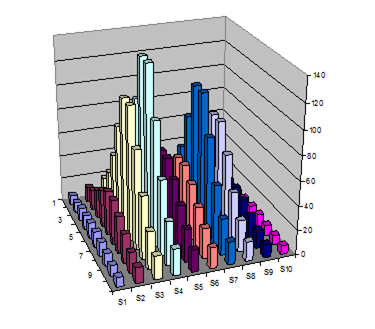
\includegraphics[width=0.9\textwidth, height=0.9\textheight, keepaspectratio=true]{media/image020.png}
\caption{3D Graph of Illuminance Map \protect \label{fig:3d-graph-of-illuminance-map}}
\end{figure}

The following figure illustrates a similar map for the tubular daylighting device example file that is included with the installation.

\begin{figure}[hbtp] % fig 9
\centering
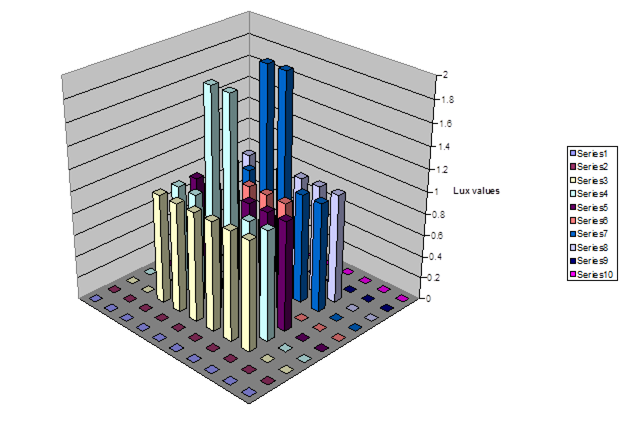
\includegraphics[width=0.9\textwidth, height=0.9\textheight, keepaspectratio=true]{media/image021.png}
\caption{A 3D illuminance map for the tubular daylighting device file \protect \label{fig:a-3d-illuminance-map-for-the-tubular}}
\end{figure}

Individual 3-D graphs can be generated for each hour of a given day and collected to generate a sequence of graphs representing the progression of daylighting conditions over the course of the day. Using additional software tools (not provided with EnergyPlus) the user can do further post-processing to link screenshots of the graphs into an animated sequence.
